% Paper A — journal-format draft (Classical and Quantum Gravity target).
% Source of truth for content: ../manuscript.md (contract-tested against the
% committed artifacts). This LaTeX rendition must not change any number,
% verdict, or claim grade; check_numbers.py enforces the number side.
% Build: ./build.sh  (XeLaTeX; Korean frozen sentences need it)
\documentclass[12pt]{article}
\usepackage{cqgmimic}

\begin{document}

% Front matter: iopart-preprint-style title block. The abstract is a
% compressed rendition of manuscript.md's (CQG limit 300 words; genre
% practice far below); every quantitative statement in it also appears,
% uncompressed, in the body.
\shorttitle{An operational reconstruction ladder from causal order}

\papertitle{An operational reconstruction ladder for spacetime quantities from causal order}

\paperauthor{Juneyoung Kim}
\paperaddress{Independent researcher}
\paperemail{lpaiu.cs@gmail.com}

\begin{paperabstract}
We study, in controlled $(1{+}1)$-dimensional (and, for dimension,
higher-dimensional) Minkowski models, which spacetime quantities can be
operationally reconstructed from a causal (accessibility) order once a
minimal, explicitly declared set of additional ingredients is supplied,
and we organize the reconstructions as a ladder. Order statistics
estimate dimension in flat Poisson-sprinkled Alexandrov intervals;
supplying a global event density turns interval cardinality into a
timelike proper-time estimate; an observer chain with clock labels
yields radar time and unsigned radar distance; an orientation reference
lifts the reflection degeneracy and recovers the Lorentz map between
inertial protocols; overlapping charts yield an approximately consistent
observer atlas; and supplied measure information makes volume
reconstruction possible under the conformal ambiguity. Three negative
results bound the ladder: causal order alone fixes no conformal scale, a
single observer yields only unsigned distance, and finite signal speed
alone does not produce Lorentzian structure; a Rindler horizon analogue
confines radar reconstruction to the expected wedge. As a preregistered
capstone we validate, on a $(3{+}1)$-dimensional vacuum plane wave whose
coordinate volume form and sprinkling law are exactly flat, that the
conformal-class information order carries is detectable at finite
density. Separate preregistered stages extend both claim classes to a
frozen Schwarzschild exterior patch (the paired claim confirmed,
single-poset discrimination detected with incomplete separation), and a
prediction-anchored stage
finds the certified-membership count of a Poisson sprinkling concordant,
within a frozen 2.5\% band, with independently certified continuum
4-volumes on each rung of a four-rung mass ladder. The contribution is
the explicit accounting of what each reconstruction requires and the
negative results that bound it; we make no claim that spacetime is
reducible to causal order.
\end{paperabstract}

\paperkeywords{causal sets, spacetime reconstruction, radar coordinates,
Poisson sprinkling, preregistered analysis}

\papersubmitto{Classical and Quantum Gravity}


\section{Introduction}\label{sec:intro}

A conservative reading of the causal-set and order-first programs is that,
for future- and past-distinguishing Lorentzian spacetimes, causal or
chronological structure determines the conformal class. Supplying a volume
element fixes the remaining conformal factor, up to diffeomorphism and unit
conventions \cite{blms1987,malament1977,hkm1976,kronheimer1967,sorkin2005,surya2019}.
This paper treats that statement operationally and quantitatively. Rather
than ask whether spacetime ``is'' a causal set, we ask: fix a causal (or
null-accessibility) order in a known model; then, supplying an explicitly
declared ingredient set, which spacetime quantities can a finite procedure
actually reconstruct, with what error, and where does each reconstruction
stop?

The value of posing it this way is an explicit \emph{ledger}. Many
individual reconstructions here are standard---proper time from longest
chains \cite{brightwell1991}, volume from interval cardinality
\cite{blms1987}, dimension from ordering fractions \cite{myrheim1978,meyer1988},
radar coordinates from an observer protocol. What is easy to lose, and what
we make explicit, is exactly which extra structure each requires and what
remains underdetermined without it. The ladder also isolates three
instructive negative results: causal order alone does not fix conformal
scale; a single observer yields only unsigned distance (a reflection
degeneracy); and finite signal speed alone does not imply Lorentzian
structure.

The contributions are: (i) a reconstruction ladder that indexes recoverable
spacetime quantities by the minimal supplied ingredient set, with per-rung
error behaviour in controlled models; (ii) grounded validations of dimension,
proper time, radar decomposition, Lorentz-map and atlas consistency, and
measure-dependent volume; (iii) three bounding negative results (conformal
scale, reflection degeneracy, finite-speed lattice); (iv) a Rindler
reconstruction-inaccessibility analogue; and (v) a preregistered
$(3{+}1)$D capstone validation that a pure-Weyl deformation of the light
cones---at identical coordinate volume form and sprinkling law---measurably
moves the causal order at finite density (\sref{sec:capstone}), together
with its type-D (Schwarzschild) extension, where separate preregistered
stages confirm the paired claim and detect single-poset discrimination
(\sref{sec:schwarzschild}); and (vi) a certified diamond-volume enclosure
and a preregistered, prediction-anchored Poisson-count validation across a
four-rung Schwarzschild mass ladder (\sref{sec:count}), with an auxiliary
instrument audit of the oracle stack (\sref{sec:oracle}). All results are
controlled validations, not evidence that geometry reduces to order.

A literature priority search (August 2026) found partial overlap in four
areas: causal-order-and-number/volume reconstruction (Braun
2025~\cite{braun2025}; Myrheim 1978~\cite{myrheim1978}; the number-volume
correspondence itself is Sorkin's~\cite{sorkin1997forks}), Schwarzschild
sprinkle-count verification (Hom\v{s}ak--Veroni~\cite{homsakveroni2024}
\S V.1), analytic diamond-volume results
(Berthiere--Gibbons--Solodukhin~\cite{berthiere2016};
Roy--Sinha--Surya~\cite{roysinhasurya2013}), and Schwarzschild
causal-relation algorithms (He--Rideout~\cite{herideout2009}; for
sprinkling-and-relations tooling more broadly,
Cunningham--Krioukov~\cite{cunninghamkrioukov2018}). The directed-rounding
volume enclosure and the preregistered equivalence gate against it appear to
have no direct precedent in that search (\sref{sec:count}); the parallel
Alfyorov--Shnyukov
estimator~\cite{alfyorov2026weyl} measures Weyl curvature from Hasse
diagrams and is taken up alongside the capstone's scope in
\sref{sec:notestablish}.

\section{The reconstruction ladder}\label{sec:ladder}

We separate the \emph{primitive} from \emph{supplied ingredients} and index
rungs by the minimal ingredient each requires.

The primitive is:
\begin{itemize}
\item \textbf{Causal / accessibility order.} A strict partial order on
  events (in the continuum models, Minkowski causal precedence;
  null-inclusive).
\end{itemize}

The supplied ingredient symbols (these form branches, not one linear
hierarchy) are:
\begin{itemize}
\item \textbf{M---global event-density calibration.} The conversion between
  event count and physical volume in the declared sampling model.
\item \textbf{O---observer chain with clock labels.} A timelike chain
  carrying ordered tick labels (an operational clock), defining a radar
  protocol.
\item \textbf{R---oriented synchronized reference.} A second beacon chain
  with calibrated separation, fixing a spatial side.
\item \textbf{A---observer atlas.} Multiple overlapping observer charts.
\item \textbf{W---local measure profile / weights.} The physical volume
  element relative to the support sampling measure, normalized to unit mean
  over the declared support, so that all scale information belongs to M and
  W carries only position dependence; a constant profile is therefore
  $\mathrm{W} = 1$ and supplies nothing beyond M.
\end{itemize}

\Tref{tab:rungs} lists the rungs (minimal ingredient $\to$ what is
reconstructed).

\begin{table}[t]
\caption{Rungs of the reconstruction ladder: the minimal ingredient set,
what it reconstructs, and what bounds it.}
\label{tab:rungs}
\begin{tabularx}{\textwidth}{@{}llXX@{}}
\toprule
Rung & Ingredient & Reconstructed & Bounded by \\
\midrule
\multicolumn{4}{@{}l}{\emph{Measure branch: order, ${+}$\,global density, ${+}$\,local measure}} \\
R0 & order only & flat-sprinkling dimension estimate; uncalibrated chain
  statistics & manifold/model assumptions; no metric scale \\
R1 & order + M & timelike proper time (interval cardinality $\to$ volume
  $\to$ $\tau$) & needs a density \\
R5 & order + M + W & volume under conformal ambiguity; coarse-graining
  stability & global and local measure supplied \\
\midrule
\multicolumn{4}{@{}l}{\emph{Observer branch: order, ${+}$\,clocked chain, ${+}$\,orientation, ${+}$\,charts}} \\
R2 & order + O & radar time; unsigned radar distance & sign undetermined \\
R3 & order + O + R & signed coordinates; Lorentz map between protocols &
  supplied orientation \\
R4 & order + O + R + A & atlas transition maps (Poincar\'e); invariant
  agreement & oriented, calibrated charts \\
\bottomrule
\end{tabularx}
\end{table}

The two branches are not of the same kind, and \tref{tab:rungs} groups
them rather than presenting six co-equal rungs. The measure branch---order,
plus a global density, plus a local measure---is the operational form of
the causal-order rigidity theorems plus a volume
element~\cite{malament1977,hkm1976}; it is where the first negative result
bites and where the whole of \sref{sec:capstone} operates. The observer
branch is protocol arithmetic: once a timelike chain with ordered tick
labels, an oriented calibrated beacon and overlapping charts have been
supplied, a coordinate system's worth of structure has been supplied, and
radar coordinates follow close to definitionally---those rungs validate
bookkeeping, and their bounding result, the reflection degeneracy, is the
protocol's own symmetry made explicit rather than a discovered obstruction.
The ledger's value is the explicit per-rung accounting; the theorem content
lives on the measure branch.

Three negative results bound the ladder from below (\sref{sec:negative}):
conformal scale is not fixed by order alone (motivating M and W); a single
observer gives only unsigned distance (motivating R); and finite signal
speed alone does not give Lorentzian structure. \Fref{fig:ladder}
summarizes the ladder.

\begin{figure}[t]
\centering
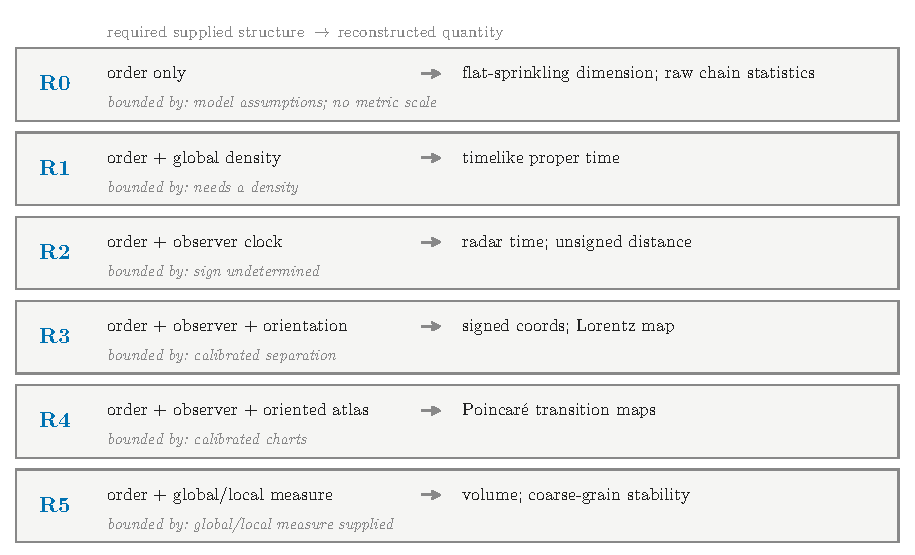
\includegraphics[width=0.95\textwidth]{figures/fig1_ladder.pdf}
\caption{The reconstruction dependency ledger. Each row names a minimal
ingredient set and the quantity it unlocks; the observer and measure rows
are branches rather than one cumulative linear chain. The ``bounded by''
line records what that ingredient set still does not supply.}
\label{fig:ladder}
\end{figure}

\section{Methods: the verified foundation layer}\label{sec:methods}

Natural units, $c = 1$. The foundation modules were checked for numerical
correctness against known results (sprinkling measure, Minkowski causal
precedence, longest-chain and interval-cardinality normalizations,
Myrheim--Meyer inversion, radar/Lorentz/Rindler formulas); this section
states the conventions the results depend on. \Fref{fig:setup} illustrates
the primitive and two of the operational constructions.

\begin{figure}[t]
\centering
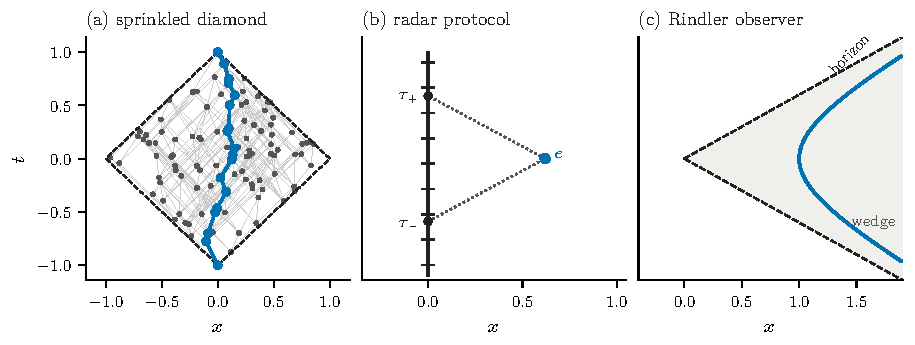
\includegraphics[width=\textwidth]{figures/fig0_setup.pdf}
\caption{The primitive and two operational constructions (illustrations
drawn with the foundation modules at a fixed seed; no measured quantity is
displayed). (a)~A Poisson sprinkling into a $(1{+}1)$D causal diamond, with
its covering (Hasse) relations in gray and one longest chain between the
diamond tips highlighted. (b)~The radar protocol: an observer chain with
tick labels, and the latest preceding ($\tau_-$) and earliest succeeding
($\tau_+$) ticks that bound a target event $e$. (c)~An accelerated
(Rindler) observer's worldline; its two-way radar reconstruction is
confined to the shaded wedge, whose boundary is the horizon.}
\label{fig:setup}
\end{figure}

\begin{itemize}
\item \textbf{Sprinkling.} Events are sampled uniformly with respect to the
  Minkowski volume in a causal diamond (rejection sampling on the
  ball-volume slice; equivalently uniform in null coordinates). The
  $(1{+}1)$D and $D$-dimensional diamonds and the $(1{+}1)$D forward cone
  are provided.
\item \textbf{Causal order.} For events $(t, x)$, $i$ precedes $j$ iff
  $t_j - t_i > 0$ and $(t_j - t_i)^2 - |x_j - x_i|^2 \ge -\texttt{atol}$
  (null-inclusive $J^+$; strict in time, so irreflexive).
\item \textbf{Longest chain.} Topological-sort longest-path dynamic
  programming on the order; the $(1{+}1)$D proper-time normalization uses
  the Brightwell--Gregory constant ($L \sim \sqrt{2\rho}\,\tau$, i.e.\
  $L \sim 2\sqrt{N}$ in a diamond of $N$ events, consistent with
  \sref{sec:r1} and appendix~\ref{app:conventions}), with an
  endpoint-inclusive counting convention and acknowledged finite-size
  corrections.
\item \textbf{Interval cardinality.} The open Alexandrov interval count $K$
  between two events estimates volume $V = K/\rho$; in $(1{+}1)$D
  $V = \tau^2/2$, so $\tau_{\mathrm{est}} = \sqrt{2K/\rho}$.
\item \textbf{Myrheim--Meyer dimension.} The ordering fraction (related
  pairs over all pairs) is inverted against the known $f(d)$ curve to
  estimate spacetime dimension in flat Alexandrov intervals.
\item \textbf{Radar coordinates.} For a supplied observer chain, $\tau_-$
  and $\tau_+$ are the latest preceding and earliest succeeding tick
  labels; radar time is their mean and radar distance their
  half-difference. A single chain gives unsigned distance; a second
  oriented chain supplies the sign. Lorentz maps between two inertial
  protocols are fit on their overlap \cite{perlick2008}.
\item \textbf{Rindler.} An accelerated (Rindler) observer in flat
  spacetime, with analytic two-way radar ticks; the reconstructible region
  is the Rindler wedge, with the horizon appearing as a
  reconstruction-inaccessibility boundary \cite{rindler1966}.
\item \textbf{Conformal / measure.} Positive conformal rescalings preserve
  causal order while changing volume and clock scale; volume reconstruction
  then requires supplied measure information (implemented in \expid{exp19}
  as local weights). In the tested random-thinning protocol, reconstruction
  is stable after density rescaling.
\end{itemize}

% Results section. Source: manuscript.md (Results).
% Every number is copied verbatim from the manuscript; do not edit digits here.
\section{Results}\label{sec:results}

Each result is a controlled validation in a known model; we report the grounded
number and its producing script.

\subsection{R0 --- order alone}\label{sec:r0}

\textbf{Dimension.} In the declared flat Poisson-sprinkling model, the
Myrheim--Meyer order statistic estimates spacetime dimension, as in earlier
tests on flat and conformally flat spacetimes~\cite{reid2003}: for true
dimension 2 the estimate moves $1.95 \to 2.03 \to 2.01 \to 1.99$ at
$N = 300$, 600, 1200, 2400; for dimension 3, $2.96 \to 2.95 \to 3.00 \to 3.00$;
for dimension 4, $4.07 \to 3.97 \to 3.93 \to 3.97$. Endpoint RMSE is lower at
$N = 2400$ than at $N = 300$, with non-monotonic finite-sample fluctuations for
dimensions 3 and 4 (\expid{exp10};
\artifact{outputs/\allowbreak{}data/\allowbreak{}dimension\_\allowbreak{}reconstruction\_\allowbreak{}summary.csv}).

\textbf{Uncalibrated timelike statistic (longest chain).} The longest chain
follows the Brightwell--Gregory scaling $L \sim \sqrt{2\rho}\,\tau$, approached
from below at finite density: at $\rho = 300$ the normalized length
$L/(\sqrt{\rho}\,\tau)$ is 1.325 with endpoints included and 1.085 with
endpoints removed, versus the asymptotic $\sqrt{2} \approx 1.414$. The
proper-time estimator reads the endpoint-exclusive length, and its mean error
there is $-0.127$; the same chains scored under the inclusive convention give
$-0.046$, the two separated by the exact offset $2/\sqrt{2\rho} = 0.082$. At
this density the median chain carries 12.5 elements including its endpoints,
so the two-element difference between the two conventions accounts for most of
that residual: at these chain lengths it is a convention effect before it is a
finite-size one (\expid{exp09};
\artifact{outputs/\allowbreak{}data/\allowbreak{}longest\_\allowbreak{}chain\_\allowbreak{}calibration\_\allowbreak{}summary.csv}). The approach
toward the asymptotic value with $N$ is shown by the chain estimator's error
falling with $N$ in \sref{sec:r1}. Raw longest-chain length is order-theoretic.
Interpreting it as proper time, including the normalization quoted here,
belongs to R1 because it requires density and a dimension-specific asymptotic
law; absolute scale is not fixed by order alone.

\subsection{R1 --- order plus measure: timelike proper time}\label{sec:r1}

With event density supplied, Alexandrov interval cardinality reconstructs
timelike proper time between internal pairs,
$\tau_{\mathrm{est}} = \sqrt{2K/\rho}$. The volume-estimator relative RMSE
falls from 0.273 at $N = 300$ to 0.105 at $N = 2400$. Its separately
aggregated RMSE is below the chain estimator's ($0.382 \to 0.231$) at every
$N$, but the volume statistic uses 500 pairs per $N$ whereas the chain
statistic uses 125, so this is not a paired comparison, and the chain
estimator additionally carries the endpoint-convention offset of
\sref{sec:r0}, so the comparison is not convention-free either
(\expid{exp07};
\artifact{outputs/\allowbreak{}data/\allowbreak{}timelike\_\allowbreak{}pair\_\allowbreak{}reconstruction\_\allowbreak{}summary.csv}). In a
fixed-interval sanity check, the interval-cardinality formula returns
$\tau = 2.0$ exactly because the full sampling diamond uses $K = N$ and
$\rho = N/V$; this is a normalization identity, not an independent accuracy
test. The chain estimate converges toward it (0.303 at $N = 200$ to 0.0125 at
$N = 2000$) (\expid{exp03};
\artifact{outputs/\allowbreak{}data/\allowbreak{}timelike\_\allowbreak{}reconstruction\_\allowbreak{}summary.csv}). The observed
errors are consistent with finite-sampling noise at the tested settings: the
ratio of reconstruction RMSE to the predicted Poisson standard deviation is
0.93--1.07 across $N$ (binomial 1.00--1.14). Smaller bias or other estimator
errors are not excluded (\expid{exp08};
\artifact{outputs/\allowbreak{}data/\allowbreak{}probe\_\allowbreak{}pair\_\allowbreak{}statistical\_\allowbreak{}calibration\_\allowbreak{}summary.csv}).

\subsection{R2 --- order plus observer: radar time and unsigned distance}\label{sec:r2}

Given an observer chain with clock labels, radar time and unsigned radar
distance are reconstructed from causal accessibility; at $N = 300$ the error
falls roughly by half per doubling of tick resolution---radar-time RMSE from
0.027 at 16 ticks to 0.0033 at 128 ticks, radar-distance RMSE from 0.071 to
0.0085, with the accessible fraction 1.0 throughout (\expid{exp11};
\artifact{outputs/\allowbreak{}data/\allowbreak{}discrete\_\allowbreak{}radar\_\allowbreak{}reconstruction\_\allowbreak{}summary.csv}). A single
observer determines only unsigned distance (the reflection degeneracy of
\sref{sec:negative}).

\subsection{R3 --- plus orientation: signed coordinates and the Lorentz map}\label{sec:r3}

A second synchronized beacon chain with known separation supplies orientation,
lifting the degeneracy to signed $(1{+}1)$D coordinates. The affine map
recovered between two oriented inertial protocols approaches the Lorentz
boost, with the fitted-$\beta$ RMSE falling with tick density. Averaged over
$N$ as in \fref{fig:convergence}, it falls from 0.00495 at 32 ticks to
0.000975 at 128 ticks for $\beta = 0.3$, and from 0.01345 to 0.00431 for
$\beta = 0.6$ (\expid{exp13};
\artifact{outputs/\allowbreak{}data/\allowbreak{}oriented\_\allowbreak{}radar\_\allowbreak{}lorentz\_\allowbreak{}summary.csv}).

\Fref{fig:convergence} collects the convergence behaviour of the first four
rungs: dimension recovery (a), timelike proper time (b), observer radar (c),
and Lorentz-map recovery (d).

\begin{figure}[t]
\centering
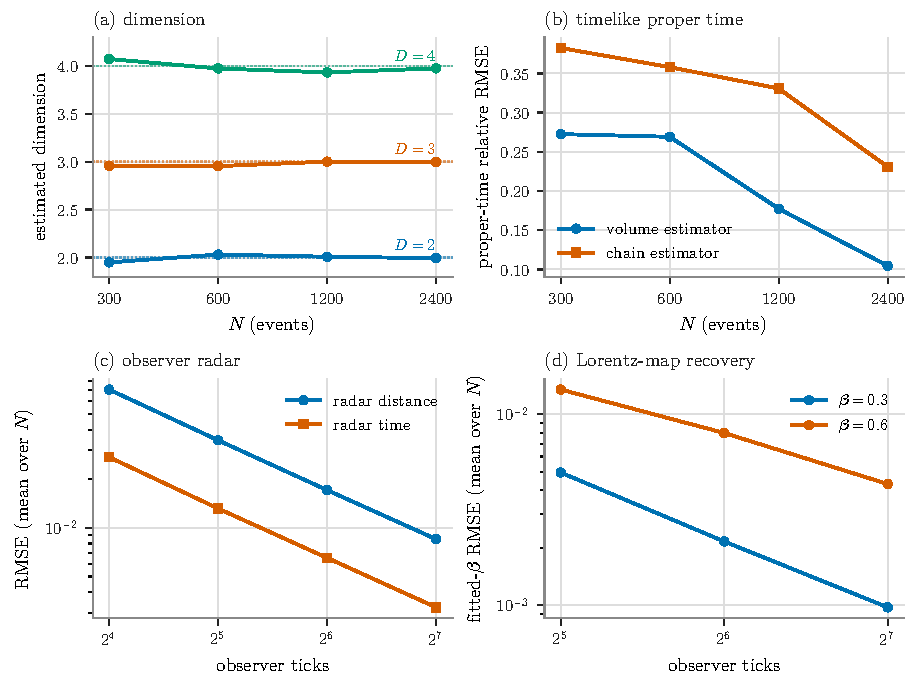
\includegraphics[width=0.95\textwidth]{figures/fig2_convergence.pdf}
\caption{Reconstruction accuracy in controlled models. (a) Myrheim--Meyer
dimension estimates lie near $D = 2$, 3, 4; endpoint RMSE is lower at
$N = 2400$ than $N = 300$ despite non-monotonic finite-sample fluctuations
(\expid{exp10}). (b) Timelike proper-time relative RMSE falls with $N$, the
interval-volume estimator below the separately aggregated longest-chain
estimator (\expid{exp07}). (c) Observer radar time and distance RMSE fall
about by half per doubling of clock ticks (\expid{exp11}). (d) Recovered
Lorentz $\beta$ RMSE falls with clock ticks for two boosts (\expid{exp13}).
Panels (c, d) are means over $N$; axes are logarithmic where noted.}
\label{fig:convergence}
\end{figure}

\subsection{R4 --- plus oriented atlas: transition-map consistency}\label{sec:r4}

With overlapping observer charts that retain the synchronized, calibrated
orientation reference from R3, affine Lorentz/Poincar\'e transition maps fit
on chart overlaps show approximately consistent composition and invariant
agreement, improving with tick density: the mean transition-map $\beta$ error
falls $0.0047 \to 0.0012$ and the invariant-interval RMSE $0.050 \to 0.010$
(ticks $32 \to 128$), while loop closure ($A \to B \to C$ versus direct
$A \to C$) has a $\beta$-composition error of $0.0072 \to 0.0017$
(\expid{exp14};
\artifact{outputs/\allowbreak{}data/\allowbreak{}observer\_\allowbreak{}atlas\_\allowbreak{}transition\_\allowbreak{}summary.csv},
\artifact{outputs/\allowbreak{}data/\allowbreak{}observer\_\allowbreak{}atlas\_\allowbreak{}loop\_\allowbreak{}summary.csv}). On exact analytic
input the same transition/loop machinery recovers the maps to machine
precision ($\beta$ error ${\sim}5.6\times10^{-17}$, RMSE
${\sim}4\times10^{-17}$) (\expid{exp15};
\artifact{outputs/\allowbreak{}data/\allowbreak{}exact\_\allowbreak{}poincare\_\allowbreak{}map\_\allowbreak{}sanity.csv}).

\subsection{R5 --- plus conformal measure: volume and coarse-graining}\label{sec:r5}

Positive conformal rescalings preserve causal order while changing volume and
clock scale: under constant (1.0/1.5/2.0) and sinusoidal rescalings the causal
matrix is unchanged and the reconstructed dimension is identical (2.020),
while the proper-time ratio tracks 1.0/1.5/2.0 and the volume ratio
1.0/2.25/4.0 (\expid{exp18};
\artifact{outputs/\allowbreak{}data/\allowbreak{}conformal\_\allowbreak{}order\_\allowbreak{}ambiguity\_\allowbreak{}summary.csv}). Two
different things must therefore be supplied, and they fail differently when
withheld: a scale (M, one number) and a shape (W, a field). The profile
\expid{exp19} tests is genuinely position-dependent---$\Omega(t) = 1 +
0.3\sin(\pi t/T)$ moves the local volume element by a factor of 3.45 across
the diamond (0.49 to 1.69) while leaving every global summary near flat: the
diamond volume moves by 2.7\% (\expid{exp18}'s sinusoidal row). A
reconstruction holding only the global density therefore has almost no bias
to correct (unweighted volume bias $-0.0057$ to $-0.0028$), but it carries a
position-dependent error that no single rescaling removes: its relative RMSE
stalls at $0.373 \to 0.298 \to 0.300$ across the tested $N$. Supplying the
local weights removes the floor: the weighted relative RMSE falls
$0.235 \to 0.176 \to 0.119$, tracking the flat-profile sampling floor
($0.234 \to 0.174 \to 0.118$) to within 1.3\%, and the
unweighted-to-weighted volume-RMSE ratio grows $2.0 \to 2.8 \to 4.3$ with
$N$---the signature of a removed systematic rather than of reduced noise.
What R5 demonstrates is the replacement of a non-vanishing error floor by
flat-case, noise-limited error scaling---a consistency statement, not a bias
correction (\expid{exp19};
\artifact{outputs/\allowbreak{}data/\allowbreak{}weighted\_\allowbreak{}conformal\_\allowbreak{}volume\_\allowbreak{}summary.csv}).

The constant-1.5 profile in the same table is a control, not the result: a
constant weight rescales estimate and truth alike, so its weighted relative
RMSE equals the flat profile's at every tested $N$, and its unweighted bias
(${\sim}{-0.29}$) is exactly the missing global factor---a normalization
identity in the sense of \sref{sec:r1}, whose repair is R1's ingredient M,
not W. The analytic volume/proper-time formulas are verified to
${\sim}1\times10^{-7}$ (\expid{exp20};
\artifact{outputs/\allowbreak{}data/\allowbreak{}conformal\_\allowbreak{}volume\_\allowbreak{}exact\_\allowbreak{}sanity.csv}). Under random
thinning, density-rescaled reconstruction is stable (volume RMSE
$0.018 \to 0.009$, dimension steady ${\sim}2.0$) while the uncorrected
estimate blows up to RMSE 0.270 (bias $-0.183$) at 25\% retention. The
thinning is uniform, so its keep probability is a single global scalar: a
robustness statement about M, not a second W-level result (\expid{exp23};
\artifact{outputs/\allowbreak{}data/\allowbreak{}thinning\_\allowbreak{}coarse\_\allowbreak{}graining\_\allowbreak{}summary.csv}). The
same measure information could be encoded in the sampling law instead of as
post-hoc weights; that variant was not run.
\Fref{fig:measure} shows the measure dependence directly.

\begin{figure}[t]
\centering
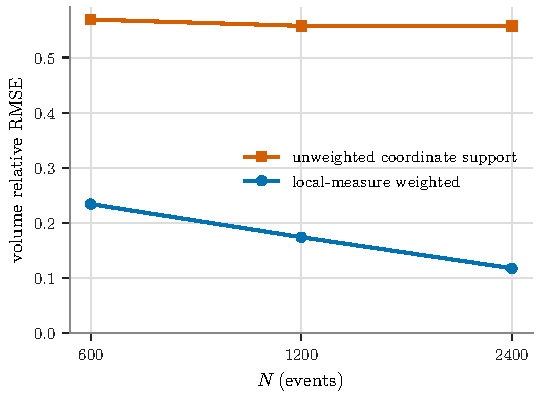
\includegraphics[width=0.95\textwidth]{figures/fig3_measure.pdf}
\caption{R5: what the local measure buys. For the position-dependent
profile, the unweighted estimate's relative error stalls at a floor that no
global recalibration removes, while the weighted estimate falls with $N$
onto the flat-profile sampling floor (a); panel (b) shows the same
comparison in absolute volume RMSE on logarithmic axes, where the two carry
visibly different slopes. The constant-profile arm is not plotted---it is a
normalization identity, R1's ingredient (\sref{sec:r5}). Order alone fixes
no absolute scale, and no scale alone fixes a profile.}
\label{fig:measure}
\end{figure}

\subsection{Horizon analogue --- Rindler reconstruction-inaccessibility}\label{sec:rindler}

For an accelerated (Rindler) observer in flat spacetime, two-way radar
reconstruction is confined to the Rindler wedge, and nothing leaks out of it:
in every configuration the classification records zero false positives and
zero false negatives, precision $=$ recall $= 1.0$. That scoring is against
the events finite clock coverage makes accessible, not against the ideal
wedge; measured against the ideal wedge the same reconstruction is incomplete,
recovering a fraction 0.74 to 0.84 of it, because part of the wedge lies
beyond the observer's tick range. The wedge itself covers about a quarter of
events (accessible fraction ${\sim}0.25$), and the in-wedge radar-time RMSE
falls with tick resolution (e.g.\ $0.0098 \to 0.0023$)
(\expid{exp16};
\artifact{outputs/\allowbreak{}data/\allowbreak{}rindler\_\allowbreak{}horizon\_\allowbreak{}reconstruction\_\allowbreak{}summary.csv}).
Comparing observers directly, all events are accessible to the inertial
observer while only ${\sim}0.25$ (ideal wedge) / ${\sim}0.21$ (finite clock
coverage) are accessible to the Rindler observer, and no event is
Rindler-accessible but inertial-inaccessible---a strict subset (\expid{exp17};
\artifact{outputs/\allowbreak{}data/\allowbreak{}inertial\_\allowbreak{}vs\_\allowbreak{}rindler\_\allowbreak{}accessibility.csv}). This is a
controlled flat-spacetime horizon analogue, not a black-hole simulation.

% Negative-results section. Source: manuscript.md (Negative results).
% Every number is copied verbatim from the manuscript; do not edit digits here.
\section{Negative results that bound the ladder}\label{sec:negative}

\begin{itemize}
\item \textbf{Conformal scale is not fixed by order alone.} Positive conformal
  rescalings leave the causal order invariant while changing physical volume
  and clock scale (\sref{sec:r5}). Absolute scale therefore requires a
  supplied measure (rung M); R0 therefore supplies uncalibrated order
  statistics, not a proper-time scale.
\item \textbf{A single observer gives only unsigned distance.} One chain's
  radar distance is $|x|$: two targets at $x = +0.1$ and $x = -0.1$ return the
  identical single-observer distance 0.1, while the two-chain oriented
  protocol recovers the signed positions $+0.1$ and $-0.1$. Signed coordinates
  therefore require an orientation reference (rung R) (\expid{exp12};
  \artifact{outputs/\allowbreak{}data/\allowbreak{}single\_\allowbreak{}observer\_\allowbreak{}reflection\_\allowbreak{}degeneracy.csv}).
\item \textbf{Finite signal speed alone does not give Lorentzian structure.}
  After calibrating density at the final time, a regular finite-speed lattice
  shares the continuum model's leading quadratic count growth, while
  finite-$t$ counts differ ($t = 5$: 21 vs 14.75; $t = 30$: 496 vs 496). Yet
  its edges lie only along the two lightcone diagonals (465 each), so it has a
  discrete symmetry, not the continuous Lorentz symmetry of a sprinkled causal
  set (\expid{exp05};
  \artifact{outputs/\allowbreak{}data/\allowbreak{}finite\_\allowbreak{}speed\_\allowbreak{}lattice\_\allowbreak{}growth.csv}). Finite speed is
  necessary but not sufficient; statistical Lorentz compatibility is the
  additional structure.
\end{itemize}

An exploratory spacelike-distance proxy (common-past / common-future /
enclosing-interval counts) is reported as boundary-dependent and \emph{not} a
validated spacelike estimator: the counts vary strongly with the sampling
region rather than tracking spacelike distance cleanly (\expid{exp06};
\artifact{outputs/\allowbreak{}data/\allowbreak{}spacelike\_\allowbreak{}distance\_\allowbreak{}proxy\_\allowbreak{}summary.csv}).

% Section 6 -- Capstone validation (manuscript.md lines 357-492).
% Numbers, verdicts, and Korean frozen sentences are copied verbatim from
% the manuscript; see ../CONVERSION.md for the binding rules.

\section{Capstone validation: finite-density detectability of the conformal class}
\label{sec:capstone}

The ladder reconstructs quantities from supplied ingredients inside flat
models; \sref{sec:negative} bounds it from below. This section caps it from
the other side, with the converse of the first negative result.
\Sref{sec:r5} showed that \emph{within} a conformal class, order carries no
scale: positive rescalings leave the causal matrix unchanged. By the theorems
that motivate the program, order determines the conformal class itself---so
\emph{across} conformal classes order must differ. Whether that difference
survives finite density, for a curvature channel that touches nothing but the
order, is the question this capstone answers affirmatively, as a
preregistered experiment (P14 in the program's internal numbering; within
this program, the first finite-density crossing of the conformal-flatness
ceiling, via a 4D type~N pure-Weyl construction).

\subsection{The \texorpdfstring{$(1{+}1)$D}{(1+1)D} conformal ceiling}
\label{sec:ceiling}

Every $(1{+}1)$D metric is conformally flat, so in the $(1{+}1)$D stages of
this program (and its curvature-focused companions P12--P13) curvature could
reach the order only through the volume-coefficient channel: those
experiments tested curvature entering through the measure/counting channel,
and the channel in which order directly carries a conformal-class difference
could not be tested there at all. This was an intended dimensional limit of
the models, not a confounded experiment: Weyl curvature---the conformal-class
content of curvature---is identically zero below four spacetime dimensions,
so a direct test needs a 4D construction built so that the measure channel is
exactly frozen while the conformal class moves.

\subsection{Pure-Weyl control construction}
\label{sec:pureweyl}

The construction is a vacuum plane wave in Brinkmann coordinates with profile
$A(u)(x^2 - y^2)$ on a constant-$A$ slab: Ricci-flat, Petrov type~N, with
$\det g = -1$ identically. Because $\det g = -1$, the coordinate volume form
and the Poisson sprinkling law are \emph{identical} to flat spacetime. That
identity supports the strongest form of pairing, and \emph{C1 uses it}: C1's
control reading is the \emph{same sprinkled point set} read with $A = 0$, so
for C1 any difference between the two readings is a functional of the
relation change alone---it cannot be a sampling artifact, an intensity
mismatch, or a calibration residual. C2 deliberately does \emph{not} pair:
its two arms are independent, unpaired sprinkling streams drawn under the
identical sprinkling law, with finite-sample variation controlled by its
frozen interval rules rather than removed by pairing---because its claim is
about telling one ensemble's posets from the other's, not about a
within-point-set counterfactual (\sref{sec:design}). What is \emph{not}
identical between geometries is the causal-diamond volume: the light-cone
boundary tilts, and at equal proper time the curved-arm diamond volume sits
0.4\% ($wT = 1$) to 7.3\% ($wT = 2$) above flat---a deterministic design
check pins both numbers, against the closed form
$V_A/V_0 = 1 + (wT)^4/252 + O((wT)^8)$. Those percentages describe a small
diamond on the axis, and the frozen operating point is neither small nor
on-axis: the probe chain selected \artifact{aniso-a1.0}, a slab spanning
$1/\pi = 0.318$ of the way to the first conjugate point, on a box elongated
three to one along the focusing transverse axis. The order statistic
therefore reads mostly off-axis pairs in the direction where the cones open,
which is why its response is a factor of three rather than a few percent.
This is a deliberately strong operating point, not a weak-curvature probe.
``Same measure'' here means the volume form and
sprinkling law only, never interval volumes; conflating the two was the first
design draft's central error, caught in review, and the distinction is
load-bearing.

\subsection{Finite-density detection design}
\label{sec:design}

An exploratory probe chain (four probes and a confirmation stage, run on seed
streams disjoint from everything that follows) selected the operating
point---slab $(1.0, 1.0, 2.0, 6.0)$, $w = 1.0$, expected 300 events per
sprinkling---and the primary statistic, the global relation fraction (the one
candidate computable from a single poset alone). The preregistered stage then
froze two claims with deliberately different boundaries, never merged into
one sentence:
\begin{itemize}
\item \textbf{C1 (paired ensemble mean).} The estimand is
  $\theta_\Delta = E[f_A - f_0]$, the ensemble mean of the \emph{net} change
  of the relation fraction over paired readings of the same points---not any
  single point set's displacement, and not the gained-plus-lost total motion.
  Confirmation requires the 95\% Student-$t$ interval of the mean paired
  difference ($n = 3000$ sprinklings) to sit entirely above a frozen margin
  $\varepsilon_\Delta = 3.579\times10^{-4}$, an operational margin anchored
  to the probe chain's confirmed block.
\item \textbf{C2 (single-poset classifier, independent replication).} A
  frozen classifier reading only the single-poset relation fraction must
  separate curved from flat ensembles ($n = 4800$ per unpaired arm) under
  three frozen interval rules (standardized separation, AUC with an exact
  boundary bound at complete separation, balanced accuracy), each with its
  own equivalence band. This claim replicates the probe chain's confirmation
  stage on fresh seeds; its failure would have been reported as a conflicting
  replication, never a retroactive cancellation.
\end{itemize}

The stage verdict POSITIVE requires both claims confirmed, certified as a
joint event before execution (4000/4000 joint-effect replicates; the null
branches certify each claim's equivalence power separately at an exact
Clopper--Pearson~\cite{clopperpearson1934} 95\% lower bound of at least 0.90; a joint equivalence
verdict is deliberately not defined, because its joint null rate sits below
that floor at the frozen sizes).

\subsection{Preregistered result}
\label{sec:preregresult}

The campaign ran once, from a clean checkout of the freeze commit, on frozen
seeds, and recorded the executing commit in the artifact. Both claims
confirmed; the stage is POSITIVE (\tref{tab:capstone}).
\Fref{fig:capstone} shows both claims.

\begin{table}[t]
\caption{Preregistered capstone verdicts. Both claims confirmed; the stage
is POSITIVE.}
\label{tab:capstone}
\centering
\begin{tabularx}{\textwidth}{@{}>{\raggedright\arraybackslash}p{9.5pc}l>{\raggedright\arraybackslash}X@{}}
\toprule
Claim & Verdict & Result (95\% CI) \\
\midrule
C1 paired ensemble mean, $n = 3000$ & confirmed &
  mean 0.0502929 $[0.0501046, 0.0504812]$; lower end $140\times$ the margin
  $3.579\times10^{-4}$ \\
C2 classifier replication, $n = 4800$/arm & confirmed &
  separation $s = 11.198$ $[11.035, 11.362]$; AUC $= 1.0$
  $[0.999232, 1.0]$; balanced accuracy $= 1.0$ $[0.986, 1.014]$ \\
\bottomrule
\end{tabularx}
\end{table}

\begin{figure}[t]
\centering
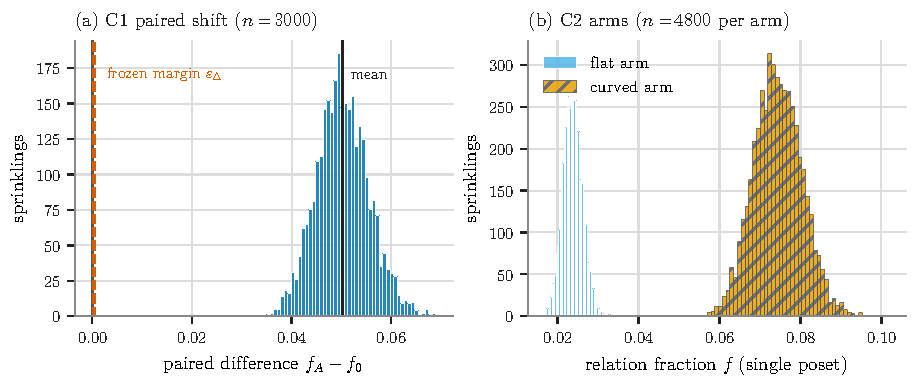
\includegraphics[width=0.95\textwidth]{figures/fig4_capstone.pdf}
\caption{(a) The distribution of the paired per-sprinkling relation-fraction
differences $f_A - f_0$ ($n = 3000$), with mean 0.0502929 (95\% CI
$[0.0501046, 0.0504812]$); the CI lower end is $140\times$ the frozen
margin $\varepsilon_\Delta = 3.579\times10^{-4}$ (marked); (b) the single-poset
relation-fraction samples of the two unpaired arms ($n = 4800$ per arm),
which are completely separated (the frozen exact-bound AUC interval is
$[0.999232, 1.0]$). Both panels are drawn from the committed artifact
(\artifact{docs/\allowbreak{}prereg/\allowbreak{}p14\_\allowbreak{}prereg\_\allowbreak{}results.json}); no value is typed in.}
\label{fig:capstone}
\end{figure}

The size of the effect is worth stating in the statistic's own units, which
the margin ratio hides: averaged over the paired readings the relation
fraction runs 0.023830 flat against 0.074123 curved, a factor of 3.11. The
two arms' relation-fraction samples are completely separated (the minimum
curved-arm value exceeds the maximum flat-arm value in 4800 draws per arm);
the AUC interval at complete separation is the frozen exact bound, not the
degenerate Wald interval. The balanced-accuracy interval got no such
treatment: its frozen construction is an unclipped Wald interval on a
worst-case standard error, so at BA $= 1.0$ it reaches 1.014, outside the
range the quantity can take. That is what the preregistration licenses and it
is printed as it stands; no verdict depends on it, because the gate reads only
the lower end. For the reader's orientation---not as a re-scored gate---the
construction the later S5 stage uses for the same quantity, a
Clopper--Pearson interval per arm combined across the two, gives
$[0.998176, 1.0]$ on the same test halves. Every relation census in both
claims recorded zero
ambiguous and zero escalated pairs. The two sentences the stage licenses were
fixed in the preregistration before execution and are recorded in the
artifact; in translation they are C1, \emph{the paired ensemble mean shift
exceeds $\varepsilon_\Delta$}, and C2, \emph{the probe chain's separation is
independently reproduced}
(\artifact{docs/\allowbreak{}prereg/\allowbreak{}p14\_\allowbreak{}prereg\_\allowbreak{}results.json};
appendix~\ref{app:provenance} records the language of the frozen originals
and what holds these renderings to them).

\subsection{What this establishes}
\label{sec:establishes}

At a fixed box, density, and profile, an order-only statistic separates flat
from curved ensembles: the conformal-class information that order carries by
theorem is \emph{present in the order at finite density}, in the one
construction where the sprinkling measure is exactly frozen. The claim is
existence, not sensitivity. No density or amplitude sweep was run, so nothing
here locates the point at which the separation would fail, and the operating
point was chosen to be strong (\sref{sec:pureweyl}) rather than marginal.
Together with \sref{sec:r5} this
closes the conformal story in both directions---within a class, order is
blind to scale; across classes, at least at this operating point, order
visibly moves.

\subsection{What the plane-wave result alone does not establish}
\label{sec:notestablish}

It says nothing about sensitivity. The frozen operating point was chosen to
be strong, and two things follow that the stage cannot answer: no density or
amplitude sweep was run, so the density at which the separation fails is
unmeasured; and the slab is elongated three to one along the focusing
transverse axis, so whether the effect survives at an isotropic box is
untested. Beyond that, it is not a general-Weyl discriminator (the plane wave
is Petrov type~N and its exact volume form is unrepresentative); it is not
Weyl-tensor recovery
(detection and recovery are different claims; no reconstructed quantity is
produced, which is why this is a capstone boundary experiment and not a new
ladder rung); it does not establish box- or density-independence (the
licensed sentence is bound to the frozen operating point); and, by itself, it
does not open the Schwarzschild generalization. Both claim classes are
carried there by the separate preregistered extensions of
\sref{sec:schwarzschild}---the C1 paired claim confirmed, C2 single-poset
discrimination detected with incomplete separation; the diamond-volume
oracle is now certified, and its direct-MC instrument audit is complete as an
auxiliary result (\sref{sec:limitations}, appendix~\ref{app:provenance}), and
the prediction-anchored Poisson-count stage is executed across a four-rung
mass ladder, CONCORDANT at every rung (\sref{sec:count}). A separate cost
measurement (S1) prices the causal-predicate component---about 0.77~ms per
pair on the tested solver, patch, and tolerance, roughly $360\times$ the
plane-wave predicate (\artifact{docs/\allowbreak{}prereg/\allowbreak{}p14\_\allowbreak{}s1\_\allowbreak{}cost.json}).

% 6.7 -- converted from manuscript.md lines 494-595 (source of truth).
\subsection{Type-D extension: preregistered C1-paired confirmation and C2-unpaired detection in Schwarzschild}\label{sec:schwarzschild}

The paired half of the capstone design transfers to the Schwarzschild
exterior on a measure identity: in Schwarzschild coordinates the volume
element is $\sqrt{-g} = r^2 \sin\theta$---independent of the mass and equal
to the flat spherical element---so one sprinkle of a coordinate patch serves
both geometries, exactly as $\det g = -1$ served the plane wave. What the
identity controls is the sampling measure; individual diamond volumes differ
under the two causal structures, and that difference is part of the signal
(the \sref{sec:pureweyl} distinction, unchanged). The frozen patch is the S1
solver domain ($M = 1$, exterior shell $r \in [10, 20]$, polar cap,
coordinate-time extent 40), with $N \sim \mathrm{Poisson}(300)$ events per
reading and the S1 predicate at tolerance $1\times10^{-8}$ with escalation
to $1\times10^{-10}$.

An exploration stage (S3, seed-ledger disciplined, preserved with its raw
per-reading arrays) measured the paired shift and sized a preregistered
confirmation (S4). The frozen rule
(\artifact{docs/\allowbreak{}prereg/\allowbreak{}p14\_\allowbreak{}s4\_\allowbreak{}schwarzschild\_\allowbreak{}c1.md}) fixes two gates
evaluated on identified intervals with strict comparisons: a primary
detection gate (identified CI95 above the frozen threshold
$\varepsilon_{\mathrm{det}} = 0.0036$, about 10\% of the exploration anchor,
in the frozen negative direction) and a secondary replication gate (the
independent two-sample Welch CI95 of the S4$-$S3 difference inside
$\pm\varepsilon_{\mathrm{rep}} = \pm 0.0012$, one exploration reading-SD); a
verified inclusion makes the joint verdict numerically equivalent to the
replication gate at these margins. Branch powers were certified before the
freeze by resampling both blocks from a conservatively scaled empirical
distribution (20000/20000 on every branch, exact Clopper--Pearson 95\% lower
bound 0.9998), with a constructed negative-control battery proving each gate
can fail. The campaign ran once, from the exact freeze checkout, with an
8-file content-addressed manifest verified at entry and at exit; the frozen
gates and results are in \tref{tab:s4}.

\begin{table}[t]
\caption{S4 frozen gates and results.}
\label{tab:s4}
\centering
\footnotesize
\begin{tabular}{@{}>{\raggedright\arraybackslash}p{6.5pc}>{\raggedright\arraybackslash}p{10pc}>{\raggedright\arraybackslash}p{11pc}>{\raggedright\arraybackslash}p{5.5pc}@{}}
\toprule
Gate & Frozen condition & Result & Verdict \\
\midrule
A: C1 detection (primary) & identified CI95 top $< -0.0036$ & CI95 $[-0.036211,\, -0.035953]$ & pass ($10\times$ margin) \\
B: replication (secondary) & Welch CI95 of S4$-$S3 inside $\pm 0.0012$ & $[-0.000183,\, +0.000194]$ & REPLICATED \\
\bottomrule
\end{tabular}
\end{table}

Stage verdict: CONFIRMED. The census recorded zero ambiguous pairs and one
escalated pair, resolved at the tighter tolerance. The frozen sentences are
recorded in Korean in the artifact
(\artifact{docs/\allowbreak{}prereg/\allowbreak{}p14\_\allowbreak{}s4\_\allowbreak{}results.json}) and quoted verbatim
(byte-exact with the artifact), each followed by a non-frozen English
translation:
``동결된 Schwarzschild 좌표·도메인(M=1, r∈[10,20], 극관각 캡 1.0, T=40)의 공통 측도 위에서, paired 앙상블 평균 이동의 identified CI95가 동결 방향으로 검출문턱 ε\_det = 0.0036을 초과했다 — 유한밀도 인과 census가 type D 진공 곡률의 빛원뿔 변형을 C1-급으로 검출했다(프로그램 내부 진술).''
(\textit{on the frozen Schwarzschild coordinates and domain, the paired
ensemble mean shift exceeds the frozen detection threshold in the frozen
direction---a finite-density causal census detects the light-cone
deformation of type-D vacuum curvature at C1 grade; a program-internal
statement});
``S4 블록과 S3 탐색 블록의 독립 두-표본 차이의 identified Welch CI95가 ±ε\_rep = ±0.0012 안에 들어, 탐색 효과가 정량적으로 재현됐다.''
(\textit{the independent two-sample difference between the S4 and S3 blocks
lies inside the replication band: the exploration effect is quantitatively
reproduced}).

A second, separate preregistered stage (S5) carries the single-poset claim
class. Guided by a committed stored-data feasibility audit
(\artifact{docs/\allowbreak{}prereg/\allowbreak{}p14\_\allowbreak{}c2\_\allowbreak{}feasibility\_\allowbreak{}audit.json}, exploratory, zero
additional solver calls, conservatively anchored), its rule
(\artifact{docs/\allowbreak{}prereg/\allowbreak{}p14\_\allowbreak{}s5\_\allowbreak{}schwarzschild\_\allowbreak{}c2.md}) declares---before
sizing and independently of the confirmation data---AUC 0.60 as the minimum
practically useful single-poset discrimination. Two \emph{independent} arms
(fresh Schwarzschild and fresh flat sprinkles; 300 readings each by a
pre-declared minimum-$n$ rule with directly certified branch powers) score
each reading by its global relation fraction; the primary gate is an
unclipped DeLong~\cite{delong1988} AUC CI95 with a four-way outcome (detected /
equivalent-at-margin / direction-reversed / inconclusive, strict
comparisons, identified-agreement across the curved bound series), and a
secondary out-of-sample balanced-accuracy gate uses a deterministic
Clopper--Pearson--Bonferroni interval with a train-half-only threshold. The
campaign ran once from its own exact freeze checkout; the frozen gates and
results are in \tref{tab:s5}.

\begin{table}[t]
\caption{S5 frozen gates and results.}
\label{tab:s5}
\centering
\footnotesize
\begin{tabular}{@{}>{\raggedright\arraybackslash}p{8.5pc}>{\raggedright\arraybackslash}p{7pc}>{\raggedright\arraybackslash}p{11.5pc}>{\raggedright\arraybackslash}p{5.7pc}@{}}
\toprule
Gate & Frozen condition & Result & Verdict \\
\midrule
Primary: AUC (DeLong) & CI95 lower $> 0.60$ & AUC 0.9734, CI95 $[0.9630,\, 0.9837]$ & \textbf{DETECTED} \\
Secondary: out-of-sample BA & joint CI95 lower $> 0.60$ & BA 0.9033, CI95 $[0.8356,\, 0.9500]$ & pass \\
\bottomrule
\end{tabular}
\end{table}

\begin{figure}[t]
\centering
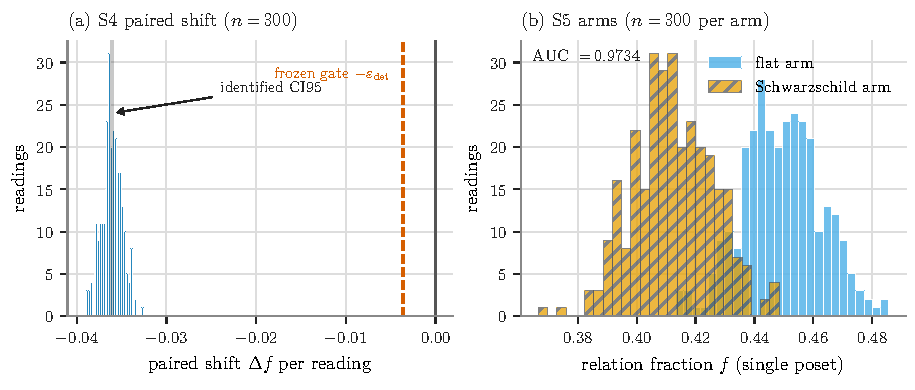
\includegraphics[width=0.95\textwidth]{figures/fig5_schwarzschild.pdf}
\caption{The Schwarzschild extension. (a)~The per-reading paired shift under
the frozen Schwarzschild domain: the identified CI95
$[-0.036211, -0.035953]$ lies an order of magnitude beyond the frozen
detection threshold $\varepsilon_{\mathrm{det}} = 0.0036$ (frozen negative
direction). (b)~The per-reading global relation fraction of the two
independent arms, discriminating with AUC 0.9734 (DeLong CI95
$[0.9630, 0.9837]$)---strong but, unlike the plane-wave C2, incomplete
separation. Drawn from the committed artifacts
(\artifact{docs/\allowbreak{}prereg/\allowbreak{}p14\_\allowbreak{}s4\_\allowbreak{}results.json},
\artifact{docs/\allowbreak{}prereg/\allowbreak{}p14\_\allowbreak{}s5\_\allowbreak{}results.json}); no value is typed in.}
\label{fig:schwarzschild}
\end{figure}

Zero ambiguous and zero escalated pairs; both identified bound series agree.
The frozen sentences are recorded in Korean in the artifact
(\artifact{docs/\allowbreak{}prereg/\allowbreak{}p14\_\allowbreak{}s5\_\allowbreak{}results.json}) and quoted verbatim
(byte-exact), each followed by a non-frozen English translation:
``동결된 Schwarzschild 도메인·밀도에서, 단일 causal set의 global relation fraction은 flat/Schwarzschild 앙상블을 우연 수준보다 판별하는 정보를 운반한다 (AUC CI95 하한 > 0.60, 프로그램 내부 진술).''
(\textit{on the frozen Schwarzschild domain and density, the global relation
fraction of a single causal set carries information that discriminates flat
from Schwarzschild ensembles above chance---AUC CI95 lower bound above 0.60;
a program-internal statement});
``out-of-sample balanced accuracy의 결합 95\% 하한이 0.60을 넘어, 학습-외 판별이 확인됐다 (secondary).''
(\textit{the joint 95\% lower bound of out-of-sample balanced accuracy
exceeds 0.60: out-of-training discrimination holds; a secondary verdict}).

What this extends, and at what grade: on the same frozen Schwarzschild
domain, the two claim classes of the plane-wave capstone are now each
supported by a \emph{separate} preregistered stage
(\fref{fig:schwarzschild})---the C1 paired claim CONFIRMED (S4), C2
single-poset discrimination DETECTED (S5). There was no joint primary
verdict, and the grades differ from the plane wave: its C2 separation was
complete, while the Schwarzschild discrimination is strong but imperfect
(AUC $\approx 0.973$; no completeness gate was preregistered); the secondary
BA verdict neither strengthens nor combines with the primary. The extension
establishes no mass-generality (a single frozen $M$) and uses no
diamond-volume oracle (margins operationally anchored or independently
declared)---the mass ladder and the certified-volume anchor belong to the
separate stage of \sref{sec:count}, which does not promote these two
verdicts. Execution provenance for both stages, including the
executed-freeze manifest snapshots---and the capstone's own freeze
ordering, mechanical gates, and commit-ancestry contract---is in
appendix~\ref{app:provenance}.

% 6.8 -- converted from manuscript.md lines 597-709 (source of truth).
\subsection{Prediction-anchored Poisson count, and its mass generalization}\label{sec:count}

Every verdict so far is anchored operationally: a margin taken from an
exploration block, or a threshold declared before sizing. This stage is
different. The diamond-volume oracle certifies an interval for the continuum
4-volume $V$ of a fixed causal diamond, by directed-rounding arithmetic and
before any count data exists; a Poisson sprinkling then supplies a count of
elements certified to lie inside that same diamond. The question is whether
the operational instrument realizes the certified prediction. Nothing in
sections~\ref{sec:capstone}--\ref{sec:schwarzschild} is used to answer it,
and the answer cannot be tuned after the fact: the endpoints, the intensity,
the tolerance and the decision rule are all frozen in the rung's
preregistration before its seed is drawn. The stage also closes a loop the
flat ladder left open: rung R1 consumed a supplied density to convert counts
into volumes, validated there against targets the same machinery produced;
here that same count-to-volume conversion---the number-volume correspondence
at the root of the causal-set program~\cite{sorkin1997forks}---is
confronted, on a Schwarzschild diamond, with a volume certified
independently of it.

\textbf{The instrument.} Points are sprinkled at a frozen intensity $A$ into
the certified box, and each point's membership is decided by the certified
causal predicate on both legs. A point the predicate cannot decide at the
frozen tolerance is \emph{not guessed}: it is counted as ambiguous
($U_{\mathrm{amb}}$) and enters the decision only through the conservative
end of the interval. Each rung first runs a fixed-$n$ ambiguity pilot (exact
Clopper--Pearson plus an exact Poisson tail bound at $\alpha = 0.01$, tail
budget $1\times10^{-3}$) that must certify $U_{\mathrm{max}} \le 30$ before
the count campaign is sized; the campaign's membership test short-circuits
on a decided first leg, so a point the campaign calls ambiguous is
necessarily one the pilot's test would also call ambiguous, and the pilot's
bound transfers \emph{a fortiori}.

\textbf{The frozen rule.} From the realized
$(K_{\mathrm{certain}}, U_{\mathrm{amb}})$ the rule builds a deliberately
conservative \emph{outer} count interval---the exact
Garwood~\cite{garwood1936} lower limit at
$K_{\mathrm{certain}}$, the upper limit at
$K_{\mathrm{certain}} + U_{\mathrm{amb}}$, each tail at level 0.025, so the
ambiguous points can only widen the interval outward and never move it
toward agreement. Rescaled by the intensity this is a volume interval
$C = [L/A, U/A]$, and the quantity gated is the \emph{identified
discrepancy} against the certified enclosure,
\begin{equation}
\begin{array}{c}
D = [C_{\mathrm{lo}} - V_{\mathrm{hi}},\; C_{\mathrm{hi}} - V_{\mathrm{lo}}],
\quad \mbox{required to lie in } [-B, +B],\\[2pt]
B = \tau V_{\mathrm{ref}}, \quad \tau = 2.5\%,
\end{array}
\end{equation}
with three ways out and no fourth: contained gives CONCORDANT, disjoint
gives DISCORDANT, and anything else gives INCONCLUSIVE, published as it
falls. The arithmetic is 96-bit end to end, and contract tests prove at the
integer boundaries that the frozen acceptance window is exactly the set of
counts the decision function calls CONCORDANT, so ``the sizing'' and ``the
verdict'' cannot drift apart. The gate is a confidence-interval form of
the two one-sided tests procedure~\cite{schuirmann1987,lakens2017} on exact
intervals, in the model-validation sense of requiring a discrepancy to fall
inside a pre-set band~\cite{robinsonfroese2004}; its statistical novelty is
the preregistered application against a certified enclosure, not the
apparatus.

\textbf{The ladder.} One rung would establish the gate at one geometry. To
ask whether the agreement is a property of the instrument rather than of a
lucky configuration, the same gate is carried across a preregistered mass
ladder. The certified shell $[10, 20]$ and the anchors $(12, 18)$ stay
fixed in \emph{absolute} coordinates, so no rung
is an isometric copy of another: the pre-frozen dimensionless indicator is
the compactness $\mu = 2M/r_c$ at the anchor midpoint $r_c = 15$, and the
executed ladder spans a factor of three in it. The mass is not the only thing
that moves, and the second motion narrows what the ladder can show. The
diamond's coordinate-time window is retuned per rung by the
frozen rule $dt(M) = 8.5\,T_{\mathrm{min}}(M)/T_{\mathrm{min}}(1)$, so that
each rung opens the same multiple of its own minimal flight time; the whole
diamond therefore scales with that flight time. The consequence is worth
stating plainly: the certified
volumes track $(dt/dt_1)^2$ to 0.007\%, 0.021\% and 0.144\% at $M = 1.4$, 1.8
and 3.0, so their mass-specific content sits one to two orders of magnitude
below the $\tau = 2.5\%$ band the gate applies. The deep end is not a free
choice either: every mass-generic lemma certifies exactly on
$M \in [0.92, 3.33]$---bounded above by the photon sphere $3M$ reaching the
shell floor at $M = 10/3$---and the deepest rung $M = 3.0$ keeps a certified
margin of a tenth of the shell floor on that binding condition---by
certification rather than by taste---its inner
anchor at $r = 4M$ between the photon sphere and the ISCO. The patch-level
lemmas are mass-generic only under stated conditions (horizon below the
shell, $K < 0$, $w$ monotone, $Q > 0$, the L2a patch bound, four L4 margins,
an L5 winding cross-check), and each is re-certified per rung as an interval
comparison---nothing is inherited silently from $M = 1$.

Four rungs were executed, each from its own exact freeze checkout, with its
own seed, once (\tref{tab:count}).

\begin{table}[t]
\caption{The four executed mass-ladder rungs: certified volume interval
$V$, pilot ambiguity outcome, sprinkled $N$, certain and ambiguous counts,
outer count interval $C$, identified discrepancy $D$, band $B$, and
verdict.}
\label{tab:count}
\centering
\scriptsize
\setlength{\tabcolsep}{2.5pt}
% Each rung occupies two physical rows: the three interval columns
% (certified V, C, D) carry their lower endpoint on the first row and
% their upper endpoint on the second, so the table fits the text width
% without shrinking below \scriptsize.
\begin{tabular}{@{}ccccccccccc@{}}
\toprule
$\mu$ & $M$ & certified $V$ & pilot & $N$ & $K_{\mathrm{certain}}$ & $U_{\mathrm{amb}}$ & $C$ & $D$ & $B$ & verdict \\
\midrule
$0.1333$ & $1.0$ & $[56.492959,$ & $k=0$ & 26,831,117 & 53,285 & 0 & $[56.205871,$ & $[-0.854796,$ & $1.419420$ & \textbf{CONCORDANT} \\
 & & $\phantom{[}57.060667]$ & & & & & $\phantom{[}57.169553]$ & $\phantom{[}{+}0.676594]$ & & \\
\addlinespace
$0.1867$ & $1.4$ & $[64.336198,$ & $k=1$ & 15,057,284 & 53,829 & 1 & $[64.307488,$ & $[-0.675256,$ & $1.616487$ & \textbf{CONCORDANT} \\
 & & $\phantom{[}64.982744]$ & & & & & $\phantom{[}65.405648]$ & $\phantom{[}{+}1.069450]$ & & \\
\addlinespace
$0.2400$ & $1.8$ & $[73.968637,$ & $k=0$ & 9,847,124 & 53,513 & 0 & $[73.695211,$ & $[-1.016709,$ & $1.858507$ & \textbf{CONCORDANT} \\
 & & $\phantom{[}74.711920]$ & & & & & $\phantom{[}74.956037]$ & $\phantom{[}{+}0.987400]$ & & \\
\addlinespace
$0.4000$ & $3.0$ & $[121.225021,$ & $k=0$ & 4,605,671 & 53,606 & 0 & $[120.802632,$ & $[-1.640649,$ & $3.045854$ & \textbf{CONCORDANT} \\
 & & $\phantom{[}122.443280]$ & & & & & $\phantom{[}122.867592]$ & $\phantom{[}{+}1.642571]$ & & \\
\bottomrule
\end{tabular}
\end{table}

\begin{figure}[t]
\centering
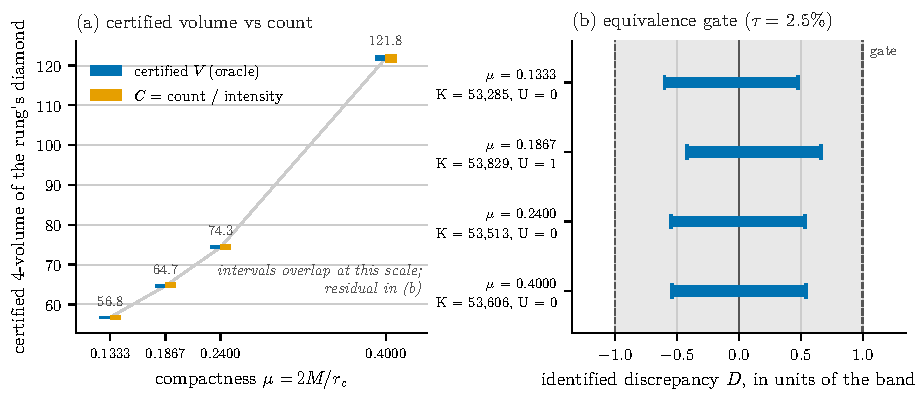
\includegraphics[width=\textwidth]{figures/fig6_ladder_count.pdf}
\caption{The executed ladder. (a)~At each preregistered compactness, the
certified continuum volume (blue) and the volume implied by the sprinkled
count (orange). The intervals overlap at plot scale across a threefold span
in $\mu$---that overlap, at each rung independently, is the result; the
cross-rung span is not itself a curvature signal (\sref{sec:count}).
(b)~The residual made visible: each
rung's identified discrepancy $D$ divided by that rung's own band
$B = \tau V_{\mathrm{ref}}$, so the rungs are comparable despite different
bands; the shaded region is the gate. Every rung is contained, with roughly
half the band to spare, and the $\mu = 0.1867$ rung's asymmetry is its
single ambiguous point widening the interval outward as the rule provides.
Both panels are generated from the same artifacts the contract tests
re-derive (\artifact{latex/\allowbreak{}figures/\allowbreak{}make\_\allowbreak{}journal\_\allowbreak{}figures.py}, reading the same artifacts as the manuscript's \artifact{figures/\allowbreak{}make\_\allowbreak{}ladder\_\allowbreak{}figure.py}); no value is typed
in.}
\label{fig:count}
\end{figure}

The certified volume grows monotonically with the compactness (57 to 65 to
74 to 122), and the realized discrepancy
stays well inside the band at every rung (\fref{fig:count}). The $M = 1.4$
pilot
returned the program's first non-zero ambiguous count ($k = 1$); it was
absorbed exactly as the sizing had provisioned, and it is visible in that
rung's asymmetric $D$, which is the conservative widening working as
designed rather than a defect.

\textbf{What this establishes.} On each preregistered rung independently, an
operational finite-density instrument realized that rung's independently
certified continuum volume to within $\tau = 2.5\%$, under a rule fixed
before the data existed. This is the first place in the program where a
measurement is confronted with a certified \emph{prediction} rather than
with an operational anchor, and the confrontation is repeated at four masses
rather than one---the deepest with its inner anchor between the photon sphere
and the ISCO. What the repetition buys is not four independent curvature
probes---the volumes are near-degenerate across rungs, as stated
above---but the re-certification of every patch-level lemma and a fresh run
of the causal predicate at each mass, none of it inherited from $M = 1$.

\textbf{What it does not establish.} The rungs are separate preregistered
stages: each verdict stands alone, there is no joint primary verdict, and no
interpolation, extrapolation, or composite cross-rung statistic is
claimed---in particular nothing is claimed at compactness between or beyond
the four tested values. Agreement of a count with a volume is not a test of
causal-set theory, and it is not evidence that spacetime is discrete; it is
a statement that this instrument, at these operating points, reproduces the
continuum measure it was pointed at. It upgrades neither the C1/C2 verdicts
of sections~\ref{sec:capstone}--\ref{sec:schwarzschild} nor the auxiliary
O4b instrument audit, none of which use it. And the result is bounded by its
construction exactly as the capstone is: one fixed diamond, one fixed
density per rung, a Schwarzschild exterior shell, and a tolerance chosen to
be feasible rather than to be sharp.

% 6.9 -- The certified volume oracle and its auxiliary instrument audit.
% Converted from manuscript.md section 6.9 (content moved there from the
% former Section 9 in the interim-review pass). Long decimals in the
% oracle/O4b passages are copied verbatim from source.
\subsection{The certified volume oracle and its auxiliary instrument audit}\label{sec:oracle}

The diamond-volume oracle behind \sref{sec:count} is fully certified: the
static-spacetime reductions derived in the public note
(\artifact{docs/\allowbreak{}theory/\allowbreak{}schwarzschild\_\allowbreak{}volume\_\allowbreak{}oracle\_\allowbreak{}note.md}) were
completed by an MPFR directed-rounding flight-time certification, a uniform
anchor-diamond containment proof, and a certified cell-refinement integrator,
and the frozen configuration's volume was computed once from an exact freeze
checkout: $V \in [56.212737, 57.348019]$, relative half-width
$0.009997 \le 0.01$, \artifact{target-met}
(\artifact{docs/\allowbreak{}prereg/\allowbreak{}p14\_\allowbreak{}o3\_\allowbreak{}volume.json}). That certification
(O3) is the one the O4b audit below consumes. O3's width would have consumed
most of the \sref{sec:count} count stage's 2.5\% band, so the same
configuration was re-certified at half the target width (O3$'$), giving
$V \in [56.492959, 57.060667]$---strictly inside O3, and the interval the
$\mu = 0.1333$ rung is gated against
(\artifact{docs/\allowbreak{}prereg/\allowbreak{}p14\_\allowbreak{}o3p\_\allowbreak{}volume.json}). The two are
distinct certifications of the same diamond at different target widths, never
combined.

An auxiliary instrument audit (O4b) then consumed that certified volume: at
the single frozen Schwarzschild configuration, the sampler, the S1 volume
response, and the certified oracle were found CONCORDANT under a frozen
composite error budget of 3.25\% with simultaneous coverage $\ge 95\%$---G1
volume interval $[56.448806185841875,$ $56.9822829864225]$ against the
certified $[56.212737, 57.348019]$ (identified discrepancy
$[-0.8992123405928396,$ $0.7695461186219887]$, band $1.7034113309135284$), G2
leak upper bound $0.14195058753928652$ within budget $0.14195094424279403$
with zero leaking points. The audit's campaign run completed both gates and
stopped at a publication-wiring defect---a software defect in the
result-publication step; no gate, seed, or datum was affected---and the
verdict was recovered by re-applying the frozen decision functions to the
preserved sufficient statistics
(\artifact{run\_\allowbreak{}kind: recovered\_\allowbreak{}completed\_\allowbreak{}campaign} in
\artifact{docs/\allowbreak{}prereg/\allowbreak{}p14\_\allowbreak{}o4b\_\allowbreak{}results.json}---no new seed, no solver call,
no resampling, no gate change), with the recovery authenticated and
bit-exactness enforced by contract tests (supplementary material,
section~S2).
This audit upgrades nothing in
sections~\ref{sec:capstone}--\ref{sec:schwarzschild}; what it is and is not
is bounded in \sref{sec:claims}. The prediction-anchored claim is carried by
the \sref{sec:count} ladder, which does not use this audit and is not
promoted by it.

% Section 7 -- Discussion. Source: ../manuscript.md section 7.
\section{Discussion}\label{sec:discussion}

The ladder is a branched accounting device, not a single cumulative
chain---and its two branches carry different kinds of content
(\sref{sec:ladder}): the measure branch the theorem content, the observer
branch protocol arithmetic. Across its dependency rows it recovers a substantial fraction of operational
Lorentzian geometry---dimension, timelike duration, radar decomposition,
Lorentz and Poincar\'e consistency, volume---from a causal order plus short,
explicit ingredient sets. It is equally a list of what each reconstruction
\emph{costs}: absolute scale costs a measure; a signed spatial coordinate
costs an orientation; a metric-not-merely-conformal statement costs a volume
element; Lorentzian structure is not bought by finite speed alone. Stating
both directions together is the point: it turns ``causal structure fixes the
conformal class, and a volume element fixes the remaining conformal factor''
from a slogan into a per-quantity operational ledger with measured error
behaviour.

This framing also clarifies what the program does \emph{not} show and sets up
the open question. Everything here is reconstruction inside known models: the
geometry is put in (by sprinkling from Minkowski or by a supplied protocol)
and recovered. It does not address whether geometry could \emph{emerge} from
an order that was not built from a geometry---the representability
question---which requires a validated discriminator and is taken up
separately. The \sref{sec:capstone} capstone sharpens the boundary from the
other side: the one piece of geometry that order itself carries---the
conformal class---is not merely present by theorem but legible to an order-only statistic at
finite density, exactly where the measure channel is frozen and only the
light cones move; how far that legibility extends before it fails is
unmeasured.

The Schwarzschild and mass-ladder stages add a second axis to that boundary.
Every verdict in the flat ladder and the plane-wave capstone is anchored
operationally---a margin taken from an exploration block, a threshold
declared before sizing. The \sref{sec:count} stage is the first
confrontation with a certified prediction instead, and what it buys is
deliberately narrow: not new physics, but the demonstration that an
operational finite-density instrument can be held to an interval-arithmetic
enclosure fixed before any data existed, at four masses, with the
near-degeneracy of the cross-rung volume comparison stated rather than
hidden. The provenance discipline that makes the confrontation
checkable---frozen decision rules, content-addressed evidence bundles,
contract tests that recompute every printed figure from its committed
artifact---is, we would argue, a contribution in its own right.

The usual scope statements are gathered here rather than in a separate
section. Results are controlled and mostly $(1{+}1)$D (dimension is checked
to 4D; the capstone and its extensions are $(3{+}1)$D). The constants are
convention-dependent (chain endpoint convention, null-inclusive causal
relation, Myrheim--Meyer normalization); we state each where it is used. The
spacelike proxy is exploratory. R5's local-measure evidence is one profile
family at one amplitude; the dose-response of the unweighted error floor to
the profile amplitude is not measured. Generalizing beyond type N is
partially opened rather than closed: the Schwarzschild extensions carry both
claim classes there (\sref{sec:schwarzschild}), and the certified oracle and
count ladder anchor the volume side (sections~\ref{sec:count}
and~\ref{sec:oracle}).

The natural next question---whether observer-relative distance \emph{order}
can be validated as recovering latent geometry, as opposed to being
reconstructed from a supplied one---is the subject of a companion paper (in
preparation) that builds a preregistered discriminator on this foundation,
measures its dose-response to geometry dilution and its dimension selection
in $(2{+}1)$D, and then carries it to orders produced by growth dynamics and
by an action-weighted 2D-order ensemble. At $N = 600$, random-start
post-burn-in configurations at $\beta = 2$ and $\beta = 8$ pass the frozen
instrument, while the $\beta = 32$ bipartite-start control is structurally
blocked (it fails at chain extraction, before any geometry gate). These are
not certified equilibrium draws, and the companion study did not establish
an equilibrium transition or finite-size scaling.

% Section 8 -- Claim boundary. Source: ../manuscript.md (index-table form,
% 2026-08-22). Full-strength claims and non-claims live in the sections the
% table points to; grade words here are copies, never restatements.
\section{Claim boundary}\label{sec:claims}

Every result in this paper is stated at full strength, with its non-claims,
in the section that establishes it; this section is the index. The
repository's \artifact{claim\_boundary.md} carries the same boundary in long
form, held to the frozen artifacts by the contract tests of
\sref{sec:repro}.

\begin{table}[t]
\caption{The claim boundary as an index. Each row names a result, the grade
at which it is claimed, the section that establishes it, and the section
that bounds it.}
\label{tab:claims}
\centering
\footnotesize
\begin{tabular}{@{}>{\raggedright\arraybackslash}p{10.5pc}>{\raggedright\arraybackslash}p{8pc}>{\raggedright\arraybackslash}p{3.6pc}>{\raggedright\arraybackslash}p{10pc}@{}}
\toprule
Result & Grade & Estab. & Bounded \\
\midrule
Flat-ladder reconstructions R0--R5 (dimension; proper time; radar time and
unsigned distance; Lorentz map; atlas; volume and its coarse-graining
stability) & controlled validations in declared models, each with its
supplied ingredients named & \S\ref{sec:r0}--\ref{sec:r5} &
\S\ref{sec:negative} \\
Rindler wedge as the reconstructible region & controlled validation; scored
against finite clock coverage & \S\ref{sec:rindler} & \S\ref{sec:rindler} \\
No absolute scale, conformal factor, signed coordinates, or unique atlas
from order alone; finite speed does not imply relativity & bounding
constructions in the stated senses & \S\ref{sec:negative} &
\S\ref{sec:negative} \\
Plane-wave capstone: paired mean under a pure-Weyl deformation (C1) and
frozen single-poset classifier (C2) & both claims confirmed; stage POSITIVE
& \S\ref{sec:preregresult} & \S\ref{sec:notestablish}: one frozen operating
point; no general-Weyl discriminator, no Weyl-tensor recovery, no box- or
density-independence \\
Schwarzschild extension: S4 paired confirmation, S5 single-poset
discrimination & CONFIRMED; DETECTED with incomplete separation &
\S\ref{sec:schwarzschild} & \S\ref{sec:schwarzschild}: separate stages, no
joint primary verdict, no mass-generality; no verdict uses the volume
oracle \\
Mass-ladder Poisson count on each of the four preregistered rungs,
$\mu \in \{0.1333$, $0.1867$, $0.2400$, $0.4000\}$ at
$\tau = 2.5\%$ & CONCORDANT at every rung, per rung & \S\ref{sec:count} &
\S\ref{sec:count}: no joint or cross-rung verdict, no interpolation, no
extrapolation; promotes no earlier verdict \\
O4b direct-MC instrument audit & CONCORDANT, auxiliary & \S\ref{sec:oracle}
& \S\ref{sec:oracle}: instrument statement only \\
\bottomrule
\end{tabular}
\end{table}

Beyond \tref{tab:claims} we claim nothing: not that spacetime is reducible
to, or emerges from, causal order; not that causal order alone yields
absolute scale, the conformal factor, signed coordinates, or a unique
atlas; not that finite signal speed implies relativity; not that any finite
validation establishes a physical theory; and, for the count stage, nothing
about causal-set theory or the discreteness of spacetime---a count agreeing
with a volume says the instrument reproduces the measure it was pointed at.
Reconstructing a geometry that was put into the model is not deriving
geometry from order.

% Section 9 -- Reproducibility. Source: manuscript.md section 9.
\section{Reproducibility}\label{sec:repro}

Foundation-layer baseline commit \texttt{325df55}. Every number in
sections~\ref{sec:results} and~\ref{sec:negative} has a cited
\artifact{experiments/\allowbreak{}exp*.py} producer and expected summary path. All 19
cited summary tables are committed under \artifact{figures/\allowbreak{}data/},
regenerated in one recorded environment (CPython 3.11.9, numpy 2.4.6,
matplotlib 3.11.1) from the unmodified baseline producers;
\artifact{artifact\_\allowbreak{}manifest.md} records the regeneration, per-file row
counts, and raw SHA-256 digests under the repository's LF storage-boundary
rule, and a contract test recomputes every digest. The submission
gate---the 19 legacy tables plus the finalized \sref{sec:capstone}
evidence bundle, provenance-locked---is met. Conventions (sprinkling
measure, causal relation, chain and interval normalizations,
Myrheim--Meyer inversion) are fixed in the foundation modules and stated
in \sref{sec:methods}.

\Sref{sec:capstone} carries no regeneration debt: every number it cites
lives in a committed artifact, and the repository's test suite recomputes
the capstone's metrics, verdicts, and sentences from the stored raw
samples, reproduces a prefix of every frozen seed stream, and asserts the
commit-ancestry contract of appendix~\ref{app:provenance}. The stage
runner (\artifact{experiments/\allowbreak{}positive\_\allowbreak{}control/\allowbreak{}p14\_\allowbreak{}prereg.py}) exposes
three modes---\texttt{preflight}, \texttt{manifest},
\texttt{campaign}---and the campaign mode refuses to run unless the
freeze manifest exists, its recorded preflight digest matches the
committed artifact, and the certified source digests match the
checked-out files.

\Sref{sec:schwarzschild} inherits the same standard for both of its
stages: each runner
(\artifact{experiments/\allowbreak{}positive\_\allowbreak{}control/\allowbreak{}s4\_\allowbreak{}schwarzschild\_\allowbreak{}c1.py},
\artifact{experiments/\allowbreak{}positive\_\allowbreak{}control/\allowbreak{}s5\_\allowbreak{}schwarzschild\_\allowbreak{}c2.py})
refuses to run unless an 8-file content-addressed freeze manifest matches
the checked-out protocol surface byte-for-byte, verified at entry and
re-verified at exit, behind a fail-closed CLI; contract tests recompute
the CONFIRMED (S4) and DETECTED (S5) verdicts---including the DeLong
interval, the balanced-accuracy threshold and
Clopper--Pearson--Bonferroni interval, and the frozen sentences---from
the stored per-reading arrays through the frozen gate functions; and the
seed ledger separates fresh allocation from deterministic replay, with
replay output owned by a separate path that can never replace a
fresh-observation artifact.

\Sref{sec:count}'s four rungs meet the same standard independently. Each
rung's ambiguity pilot and count campaign run behind their own frozen,
content-addressed manifests
(\artifact{docs/\allowbreak{}prereg/\allowbreak{}p14\_\allowbreak{}*\_\allowbreak{}count\_\allowbreak{}freeze\_\allowbreak{}manifest.json},
with the executed surfaces preserved alongside), from a clean exact
checkout recorded in the artifact at entry and exit; the per-rung runners
are \artifact{experiments/\allowbreak{}oracle/\allowbreak{}o5\_\allowbreak{}count\_\allowbreak{}campaign.py} and
\artifact{experiments/\allowbreak{}oracle/\allowbreak{}s6\_\allowbreak{}m\{14,18,30\}\_\allowbreak{}count.py}, and
\artifact{tests/\allowbreak{}test\_\allowbreak{}paper\_\allowbreak{}a\_\allowbreak{}count\_\allowbreak{}integration.py} re-derives
the printed per-rung table from the artifacts. The commit chain per rung
is in appendix~\ref{app:provenance}.

The auxiliary O4b instrument audit (\sref{sec:oracle}) meets the
same standard with one addition. Its campaign runner refuses to run
except on the clean exact checkout of the approved freeze SHA against a
25-file content-addressed manifest with an environment lock; the executed
surface is preserved byte-for-byte as
\artifact{docs/\allowbreak{}prereg/\allowbreak{}p14\_\allowbreak{}o4b\_\allowbreak{}executed\_\allowbreak{}freeze\_\allowbreak{}manifest.json}. Because
the run stopped at a publication-wiring defect after both gates
completed, the published verdict is a \emph{recovery}:
\artifact{experiments/\allowbreak{}oracle/\allowbreak{}o4b\_\allowbreak{}recover.py} re-applies the frozen
decision functions (empirical-Bernstein interval, Clopper--Pearson bound,
frozen sizing constants) to the preserved sufficient statistics,
authenticates its inputs against the SHA-256 of the committed incident
and checkpoint records with a two-file cross-check, and refuses to
publish unless the recomputation reproduces the preserved verdict
bit-for-bit; contract tests (\artifact{tests/\allowbreak{}test\_\allowbreak{}o4b\_\allowbreak{}recover.py}) pin
the recomputation, the tamper refusals, and the published artifact, and
regression tests (\artifact{tests/\allowbreak{}test\_\allowbreak{}o4b\_\allowbreak{}wiring\_\allowbreak{}fixes.py}) drive the
repaired \texttt{main()} path end to end. No new seed was drawn, no
solver called, no point resampled, and no gate changed anywhere in the
recovery.


% Back matter -- acknowledgements/disclosure (manuscript.md lines
% 1043-1089) and a CQG-style data availability statement written for the
% journal format, faithful to section 10. The manuscript's "References"
% stub is superseded by the bibliography in main.tex.
\section*{Acknowledgements and disclosure}

This work was carried out with substantial assistance from AI language
models (Anthropic Claude), used for literature search, code and
manuscript drafting, numerical analysis, and adversarial review of the
author's own claims. The AI systems are not authors and bear no
responsibility: the author takes full responsibility for every claim,
number, and citation here.

How the output was verified, and how far that verification reaches.
Every quantitative result in
sections~\ref{sec:results}--\ref{sec:count} is produced by a committed
experiment script whose output file is pinned by a content-addressed
manifest that a contract test recomputes, so the \emph{artifacts} cannot
drift unnoticed. The manuscript's own transcription of those artifacts is
machine-checked across the whole results arc: every figure printed in
sections~\ref{sec:results} through~\ref{sec:schwarzschild} is re-derived
from its artifact and matched against the sentence that prints it,
\sref{sec:count}'s per-rung table is re-derived the same way, and the
auxiliary audit's figures are pinned verbatim---so a hand-typed value
fails the build, and so does one that silently moves to a neighboring
claim. The claim list is itself guarded: every numeral in
sections~\ref{sec:results}--\ref{sec:schwarzschild} must be one the
contract derives or one it names as an accepted exclusion with a reason,
the exclusions being row selectors, rung labels and construction settings
rather than results, so a figure added later cannot slip past unchecked.
Provenance runs by two routes, both digest-locked at the artifact. The
legacy results of sections~\ref{sec:results} and~\ref{sec:negative} name
their producing experiment (\expid{exp03}--\expid{exp23}) and its
committed summary table, audited in \artifact{producer\_\allowbreak{}audit.md}. The
preregistered results of sections~\ref{sec:capstone}--\ref{sec:count}
name their own frozen artifacts---\artifact{p14\_\allowbreak{}prereg\_\allowbreak{}results.json}
for the capstone, \artifact{p14\_\allowbreak{}s4\_\allowbreak{}results.json} and
\artifact{p14\_\allowbreak{}s5\_\allowbreak{}results.json} for the Schwarzschild extensions, the
per-rung count records for \sref{sec:count}, and
\artifact{p14\_\allowbreak{}o4b\_\allowbreak{}results.json} for the auxiliary audit---each with its
executed freeze manifest. What the contract does not do is stated too: it
holds the printed characters to the committed artifact, not the artifact
to nature, it re-runs no experiment, and it reaches
sections~\ref{sec:results}--\ref{sec:count} and the auxiliary audit's
figures only; numbers quoted elsewhere in the paper are still checked by
reading. Writing it corrected two transcriptions that reading had passed
(\sref{sec:r2}'s radar-distance RMSE and \sref{sec:preregresult}'s C2
separation statistic), which is why the reach is now stated as a contract
rather than as care; the claim boundary's copies of the same figures are
held to the same artifacts, because that is where one of the two had been
copied as well. The preregistered stages ran once each from an exact
clean checkout of a merged freeze commit, under frozen decision rules,
with their verdicts computed by the frozen code rather than asserted in
prose. Every bibliographic entry was checked against an authoritative
record (arXiv, Crossref, or the publisher) and then re-checked
independently; the priority assessments in the companion records name the
sources that were fetched.

\section*{Data availability statement}

All data supporting the results of this study are version-controlled in
the public repository at
\url{https://github.com/lpaiu-cs/causal-spacetime}: the 19 digest-locked
summary tables under \artifact{figures/\allowbreak{}data/}, and the preregistered
evidence bundles and frozen artifacts of
sections~\ref{sec:capstone}--\ref{sec:count} and the auxiliary audit.
Every cited file is pinned by a content-addressed manifest whose digests
the repository's contract tests recompute.


% The former appendices (conventions; capstone execution provenance) are
% packaged as a separate supplementary-material document (si.tex, sections
% S1 and S2) per the submission plan; body references say "supplementary
% material". Re-inserting them as in-article appendices is two \input
% lines plus the appendix preamble -- see git history.

% Hand-built IOP/CQG-format numeric bibliography (Vancouver, order of first
% citation). Data source: ../citations/references.bib (verified); the entry
% order is pinned to the \citation order in main.aux — re-check it if a
% \cite is added or moved.
% thebibliography prints the References heading itself
\begin{thebibliography}{99}

\bibitem{blms1987} Bombelli L, Lee J, Meyer D and Sorkin R D 1987 Space-time as a causal set \textit{Phys. Rev. Lett.} \textbf{59} 521--4

\bibitem{malament1977} Malament D B 1977 The class of continuous timelike curves determines the topology of spacetime \textit{J. Math. Phys.} \textbf{18} 1399--404

\bibitem{hkm1976} Hawking S W, King A R and McCarthy P J 1976 A new topology for curved space-time which incorporates the causal, differential, and conformal structures \textit{J. Math. Phys.} \textbf{17} 174--81

\bibitem{kronheimer1967} Kronheimer E H and Penrose R 1967 On the structure of causal spaces \textit{Proc. Camb. Phil. Soc.} \textbf{63} 481--501

\bibitem{sorkin2005} Sorkin R D 2005 Causal sets: discrete gravity (notes for the Valdivia Summer School), in \textit{Lectures on Quantum Gravity} ed A Gomberoff and D Marolf (New York: Springer) pp 305--27 (arXiv:gr-qc/0309009)

\bibitem{surya2019} Surya S 2019 The causal set approach to quantum gravity \textit{Living Rev. Relativ.} \textbf{22} 5

\bibitem{brightwell1991} Brightwell G and Gregory R 1991 The structure of random discrete spacetime \textit{Phys. Rev. Lett.} \textbf{66} 260--3

\bibitem{myrheim1978} Myrheim J 1978 Statistical geometry \textit{Preprint} CERN-TH-2538

\bibitem{meyer1988} Meyer D A 1988 \textit{The Dimension of Causal Sets} PhD Thesis Massachusetts Institute of Technology

\bibitem{perlick2008} Perlick V 2008 On the radar method in general-relativistic spacetimes, in \textit{Lasers, Clocks and Drag-Free Control} (Astrophysics and Space Science Library vol 349) ed H Dittus, C Lammerzahl and S G Turyshev (Berlin: Springer) pp 131--52

\bibitem{rindler1966} Rindler W 1966 Kruskal space and the uniformly accelerated frame \textit{Am. J. Phys.} \textbf{34} 1174--8

\bibitem{clopperpearson1934} Clopper C J and Pearson E S 1934 The use of confidence or fiducial limits illustrated in the case of the binomial \textit{Biometrika} \textbf{26} 404--13

\bibitem{delong1988} DeLong E R, DeLong D M and Clarke-Pearson D L 1988 Comparing the areas under two or more correlated receiver operating characteristic curves: a nonparametric approach \textit{Biometrics} \textbf{44} 837--45

\bibitem{garwood1936} Garwood F 1936 Fiducial limits for the Poisson distribution \textit{Biometrika} \textbf{28} 437--42

\bibitem{braun2025} Braun M 2025 Spacetime reconstruction by order and number (arXiv:2507.01907)

\bibitem{homsakveroni2024} Hom\v{s}ak V and Veroni S 2024 Boltzmannian state counting for black hole entropy in Causal Set Theory (arXiv:2404.11670)

\bibitem{berthiere2016} Berthiere C, Gibbons G and Solodukhin S N 2016 Comparison theorems for causal diamonds \textit{Nucl. Phys.} B \textbf{904} 494--508

\bibitem{herideout2009} He S and Rideout D 2009 A causal set black hole \textit{Class. Quantum Grav.} \textbf{26} 125015

\bibitem{alfyorov2026weyl} Alfyorov D and Shnyukov I 2026 Weyl curvature from the Hasse diagram: a parameter-free bridge formula for causal sets (Zenodo) DOI: 10.5281/zenodo.19364212

\bibitem{schuirmann1987} Schuirmann D J 1987 A comparison of the two one-sided tests procedure and the power approach for assessing the equivalence of average bioavailability \textit{J. Pharmacokinet. Biopharm.} \textbf{15} 657--80

\bibitem{lakens2017} Lakens D 2017 Equivalence tests: a practical primer for $t$ tests, correlations, and meta-analyses \textit{Soc. Psychol. Personal. Sci.} \textbf{8} 355--62

\bibitem{robinsonfroese2004} Robinson A P and Froese R E 2004 Model validation using equivalence tests \textit{Ecol. Model.} \textbf{176} 349--58

\end{thebibliography}


\end{document}
